\documentclass{standalone}
\usepackage{tikz}
\usepackage{ctex,siunitx}
\setCJKmainfont{Noto Serif CJK SC}
\usepackage{tkz-euclide}
\usepackage{amsmath}
\usetikzlibrary{patterns, calc}
\usetikzlibrary {decorations.pathmorphing, decorations.pathreplacing, decorations.shapes,}

\begin{document}
\small
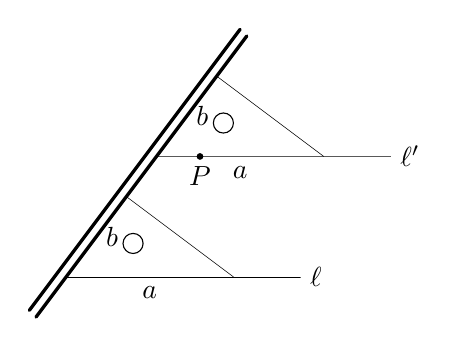
\begin{tikzpicture}[>=stealth,scale=0.85]
  \tkzSetUpPoint[fill=black]
  % \useasboundingbox(-1,-0.75)rectangle(3.7,1.4);
  \tkzDefPoints{0/0/A, 3.5/0/D, 2.5/0/B, .9/1.2/C, 1/.5/O}
  \tkzDefPointWith[linear, K=1.5](A,C)\tkzGetPoint{A'}      
  \tkzDefPointsBy[translation = from A to A'](B,C,D,O){B',C',D',O'}
  \draw(O) circle(.15);
  \draw(O') circle(.15);
  \tkzDrawSegments(A,D B,C A,C)
  \tkzDrawSegments(A',D' B',C' A',C')
  \tkzLabelPoint[right](D){$\ell$}
  \tkzLabelPoint[right](D'){$\ell'$}
  \tkzDrawLines[very thick](A,C')
  \tkzDefPoints{-.1/.1/a}
  \tkzDefPointsBy[translation = from A to a](C'){c}
  \tkzDrawLines[very thick](a,c)
  \tkzLabelSegment[below](A,B){$a$};
  \tkzLabelSegment[below](A',B'){$a$};
  \tkzLabelSegment[right](A,C){$b$};
  \tkzLabelSegment[right](A',C'){$b$};
  \tkzDefPoints{2/1.8/P}
  \tkzDrawPoints(P)
  \tkzLabelPoints[below](P)
\end{tikzpicture}
\end{document}